% Options for packages loaded elsewhere
% Options for packages loaded elsewhere
\PassOptionsToPackage{unicode}{hyperref}
\PassOptionsToPackage{hyphens}{url}
\PassOptionsToPackage{dvipsnames,svgnames,x11names}{xcolor}
%
\documentclass[
  letterpaper,
  DIV=11,
  numbers=noendperiod]{scrreprt}
\usepackage{xcolor}
\usepackage{amsmath,amssymb}
\setcounter{secnumdepth}{5}
\usepackage{iftex}
\ifPDFTeX
  \usepackage[T1]{fontenc}
  \usepackage[utf8]{inputenc}
  \usepackage{textcomp} % provide euro and other symbols
\else % if luatex or xetex
  \usepackage{unicode-math} % this also loads fontspec
  \defaultfontfeatures{Scale=MatchLowercase}
  \defaultfontfeatures[\rmfamily]{Ligatures=TeX,Scale=1}
\fi
\usepackage{lmodern}
\ifPDFTeX\else
  % xetex/luatex font selection
\fi
% Use upquote if available, for straight quotes in verbatim environments
\IfFileExists{upquote.sty}{\usepackage{upquote}}{}
\IfFileExists{microtype.sty}{% use microtype if available
  \usepackage[]{microtype}
  \UseMicrotypeSet[protrusion]{basicmath} % disable protrusion for tt fonts
}{}
\makeatletter
\@ifundefined{KOMAClassName}{% if non-KOMA class
  \IfFileExists{parskip.sty}{%
    \usepackage{parskip}
  }{% else
    \setlength{\parindent}{0pt}
    \setlength{\parskip}{6pt plus 2pt minus 1pt}}
}{% if KOMA class
  \KOMAoptions{parskip=half}}
\makeatother
% Make \paragraph and \subparagraph free-standing
\makeatletter
\ifx\paragraph\undefined\else
  \let\oldparagraph\paragraph
  \renewcommand{\paragraph}{
    \@ifstar
      \xxxParagraphStar
      \xxxParagraphNoStar
  }
  \newcommand{\xxxParagraphStar}[1]{\oldparagraph*{#1}\mbox{}}
  \newcommand{\xxxParagraphNoStar}[1]{\oldparagraph{#1}\mbox{}}
\fi
\ifx\subparagraph\undefined\else
  \let\oldsubparagraph\subparagraph
  \renewcommand{\subparagraph}{
    \@ifstar
      \xxxSubParagraphStar
      \xxxSubParagraphNoStar
  }
  \newcommand{\xxxSubParagraphStar}[1]{\oldsubparagraph*{#1}\mbox{}}
  \newcommand{\xxxSubParagraphNoStar}[1]{\oldsubparagraph{#1}\mbox{}}
\fi
\makeatother


\usepackage{longtable,booktabs,array}
\usepackage{calc} % for calculating minipage widths
% Correct order of tables after \paragraph or \subparagraph
\usepackage{etoolbox}
\makeatletter
\patchcmd\longtable{\par}{\if@noskipsec\mbox{}\fi\par}{}{}
\makeatother
% Allow footnotes in longtable head/foot
\IfFileExists{footnotehyper.sty}{\usepackage{footnotehyper}}{\usepackage{footnote}}
\makesavenoteenv{longtable}
\usepackage{graphicx}
\makeatletter
\newsavebox\pandoc@box
\newcommand*\pandocbounded[1]{% scales image to fit in text height/width
  \sbox\pandoc@box{#1}%
  \Gscale@div\@tempa{\textheight}{\dimexpr\ht\pandoc@box+\dp\pandoc@box\relax}%
  \Gscale@div\@tempb{\linewidth}{\wd\pandoc@box}%
  \ifdim\@tempb\p@<\@tempa\p@\let\@tempa\@tempb\fi% select the smaller of both
  \ifdim\@tempa\p@<\p@\scalebox{\@tempa}{\usebox\pandoc@box}%
  \else\usebox{\pandoc@box}%
  \fi%
}
% Set default figure placement to htbp
\def\fps@figure{htbp}
\makeatother


% definitions for citeproc citations
\NewDocumentCommand\citeproctext{}{}
\NewDocumentCommand\citeproc{mm}{%
  \begingroup\def\citeproctext{#2}\cite{#1}\endgroup}
\makeatletter
 % allow citations to break across lines
 \let\@cite@ofmt\@firstofone
 % avoid brackets around text for \cite:
 \def\@biblabel#1{}
 \def\@cite#1#2{{#1\if@tempswa , #2\fi}}
\makeatother
\newlength{\cslhangindent}
\setlength{\cslhangindent}{1.5em}
\newlength{\csllabelwidth}
\setlength{\csllabelwidth}{3em}
\newenvironment{CSLReferences}[2] % #1 hanging-indent, #2 entry-spacing
 {\begin{list}{}{%
  \setlength{\itemindent}{0pt}
  \setlength{\leftmargin}{0pt}
  \setlength{\parsep}{0pt}
  % turn on hanging indent if param 1 is 1
  \ifodd #1
   \setlength{\leftmargin}{\cslhangindent}
   \setlength{\itemindent}{-1\cslhangindent}
  \fi
  % set entry spacing
  \setlength{\itemsep}{#2\baselineskip}}}
 {\end{list}}
\usepackage{calc}
\newcommand{\CSLBlock}[1]{\hfill\break\parbox[t]{\linewidth}{\strut\ignorespaces#1\strut}}
\newcommand{\CSLLeftMargin}[1]{\parbox[t]{\csllabelwidth}{\strut#1\strut}}
\newcommand{\CSLRightInline}[1]{\parbox[t]{\linewidth - \csllabelwidth}{\strut#1\strut}}
\newcommand{\CSLIndent}[1]{\hspace{\cslhangindent}#1}



\setlength{\emergencystretch}{3em} % prevent overfull lines

\providecommand{\tightlist}{%
  \setlength{\itemsep}{0pt}\setlength{\parskip}{0pt}}



 


\usepackage{booktabs}
\usepackage{caption}
\usepackage{longtable}
\usepackage{colortbl}
\usepackage{array}
\usepackage{anyfontsize}
\usepackage{multirow}
\KOMAoption{captions}{tableheading}
\makeatletter
\@ifpackageloaded{tcolorbox}{}{\usepackage[skins,breakable]{tcolorbox}}
\@ifpackageloaded{fontawesome5}{}{\usepackage{fontawesome5}}
\definecolor{quarto-callout-color}{HTML}{909090}
\definecolor{quarto-callout-note-color}{HTML}{0758E5}
\definecolor{quarto-callout-important-color}{HTML}{CC1914}
\definecolor{quarto-callout-warning-color}{HTML}{EB9113}
\definecolor{quarto-callout-tip-color}{HTML}{00A047}
\definecolor{quarto-callout-caution-color}{HTML}{FC5300}
\definecolor{quarto-callout-color-frame}{HTML}{acacac}
\definecolor{quarto-callout-note-color-frame}{HTML}{4582ec}
\definecolor{quarto-callout-important-color-frame}{HTML}{d9534f}
\definecolor{quarto-callout-warning-color-frame}{HTML}{f0ad4e}
\definecolor{quarto-callout-tip-color-frame}{HTML}{02b875}
\definecolor{quarto-callout-caution-color-frame}{HTML}{fd7e14}
\makeatother
\makeatletter
\@ifpackageloaded{bookmark}{}{\usepackage{bookmark}}
\makeatother
\makeatletter
\@ifpackageloaded{caption}{}{\usepackage{caption}}
\AtBeginDocument{%
\ifdefined\contentsname
  \renewcommand*\contentsname{Table of contents}
\else
  \newcommand\contentsname{Table of contents}
\fi
\ifdefined\listfigurename
  \renewcommand*\listfigurename{List of Figures}
\else
  \newcommand\listfigurename{List of Figures}
\fi
\ifdefined\listtablename
  \renewcommand*\listtablename{List of Tables}
\else
  \newcommand\listtablename{List of Tables}
\fi
\ifdefined\figurename
  \renewcommand*\figurename{Figure}
\else
  \newcommand\figurename{Figure}
\fi
\ifdefined\tablename
  \renewcommand*\tablename{Table}
\else
  \newcommand\tablename{Table}
\fi
}
\@ifpackageloaded{float}{}{\usepackage{float}}
\floatstyle{ruled}
\@ifundefined{c@chapter}{\newfloat{codelisting}{h}{lop}}{\newfloat{codelisting}{h}{lop}[chapter]}
\floatname{codelisting}{Listing}
\newcommand*\listoflistings{\listof{codelisting}{List of Listings}}
\makeatother
\makeatletter
\makeatother
\makeatletter
\@ifpackageloaded{caption}{}{\usepackage{caption}}
\@ifpackageloaded{subcaption}{}{\usepackage{subcaption}}
\makeatother
\usepackage{bookmark}
\IfFileExists{xurl.sty}{\usepackage{xurl}}{} % add URL line breaks if available
\urlstyle{same}
\hypersetup{
  pdftitle={Project Sharknado: Evaluating the Risk of Coastal-Origin Tornadoes in the United States},
  pdfauthor={Sophia Heinrich},
  colorlinks=true,
  linkcolor={blue},
  filecolor={Maroon},
  citecolor={Blue},
  urlcolor={Blue},
  pdfcreator={LaTeX via pandoc}}


\title{Project Sharknado: Evaluating the Risk of Coastal-Origin
Tornadoes in the United States}
\author{Sophia Heinrich}
\date{}
\begin{document}
\maketitle

\renewcommand*\contentsname{Table of contents}
{
\hypersetup{linkcolor=}
\setcounter{tocdepth}{2}
\tableofcontents
}

\bookmarksetup{startatroot}

\chapter*{Executive Summary}\label{executive-summary}
\addcontentsline{toc}{chapter}{Executive Summary}

\markboth{Executive Summary}{Executive Summary}

\begin{figure}

\centering{

\pandocbounded{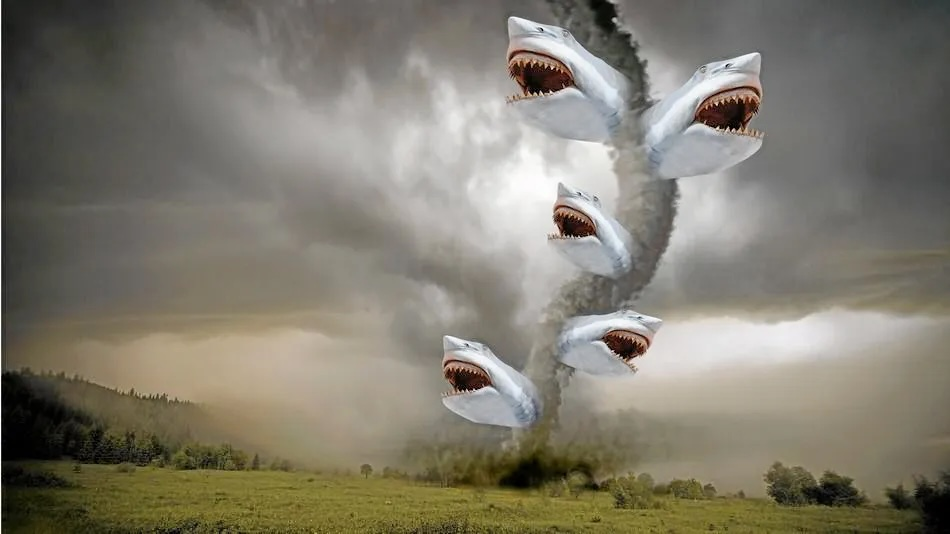
\includegraphics[keepaspectratio]{assets/sharknado.jpeg}}

}

\caption{\label{fig-sharknado}This is a fictional mockup of what a
sharknado could look like if they were actually real.}

\end{figure}%

\section*{Purpose of Report}\label{purpose-of-report}
\addcontentsline{toc}{section}{Purpose of Report}

\markright{Purpose of Report}

The insurance agency has seen a rise in property payouts driven by the
intensifying effects of climate change on extreme weather. In the wake
of the `Sharknado' phenomenon sparked by the 2013 film, the agency is
now investigating whether the increasing frequency of severe weather
could lead to a higher likelihood of shark-infested weather events (as
depicted in Figure~\ref{fig-sharknado}). The purpose of this report is
to

\begin{itemize}
\tightlist
\item
  \textbf{Determine the likelihood of sharknadoes forming.}
\item
  \textbf{Determine the economic impact of sharknadoes.}
\end{itemize}

\section*{Background}\label{background}
\addcontentsline{toc}{section}{Background}

\markright{Background}

Historically, the majority of tornadoes have occurred in the Central
United States, a region nicknamed ``Tornado Alley''. Since this region
is not near any coasts, the plausibility of a tornado picking up a shark
out of coastal waters is low. However, there have been a few recorded
tornadoes near the coast, leading the agency to wonder if sharknadoes
are not an impossibility.

While there has not been any formal scientific literature that has
studied the likelihood and impacts of tornadoes carrying sharks, one
scholar, Dr.~Kim Martini, entertained the idea and provided an analysis
on the likelihood of a sharknado with her knowledge in marine biology
and physics. Through logical reasoning, Martini concluded that while a
typical tornado travels over enough geographic area and can be strong
enough to keep a shark airborne, it is highly unlikely that a tornado
could lift the shark out of the water in the first place.

For the sake of still conducting a statistical analysis, this report
ignores this physical impossibility.

\section*{Methods}\label{methods}
\addcontentsline{toc}{section}{Methods}

\markright{Methods}

75 years of tornado storm data (1950-2025) from the National Weather
Service was analyzed to assess the likelihood and economic impact of a
sharknado. After cleaning the data, a total of 31,345 storms were
classified by path trajectory and shark-lifting potential (based on the
Fujita scale) and analyzed for sharknado-likeness and total property
damage.

A tornado's \emph{path trajectory} was classified as one of three labels
(see Figure~\ref{fig-path-trajectories}):

\begin{figure}

\centering{

\pandocbounded{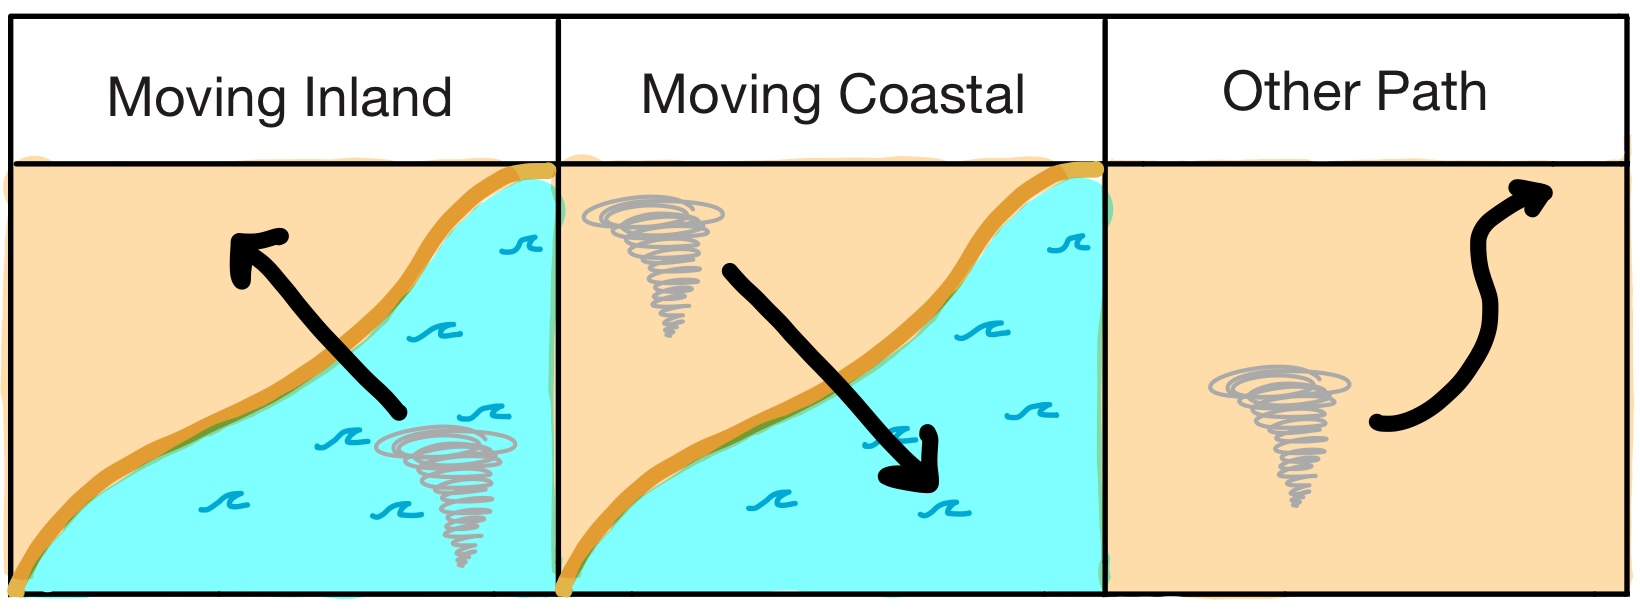
\includegraphics[keepaspectratio]{assets/path-trajectories.jpeg}}

}

\caption{\label{fig-path-trajectories}This is a diagram illustrating the
movement of tornadoes relative to the coast and inland, with path
trajectory labels of ``Moving Inland'', ``Moving Coastal'', and ``Other
Path''.}

\end{figure}%

A tornado's \emph{shark-lifting potential} was classified as one of two
labels:

\begin{itemize}
\tightlist
\item
  \textbf{Low Potential}: tornado was given an F1 or F2 rating on the
  (Enhanced) Fujita Scale
\item
  \textbf{High Potential}: tornado was given an F3, F4, or F5 rating on
  the (Enhanced) Fujita Scale
\end{itemize}

\section*{Findings \& Conclusions}\label{findings-conclusions}
\addcontentsline{toc}{section}{Findings \& Conclusions}

\markright{Findings \& Conclusions}

Throughout the analysis, storms classified as ``Moving Inland'' and
``High {[}shark-lifting{]} Potential'' were of the highest interest as
they exhibit characteristics most similar to a sharknado. Of the 31,345
recorded storms, only 2 were classified as both ``Moving Inland'' and
``High Potential'' for lifting sharks. While the Atlantic and Gulf
coasts were the primary region of origin for ``Moving Inland'' storms,
these events statistically lacked the same shark-lifting potential of
storms originating inland. In terms of economic impacts, ``Moving
Inland'' storm with high shark-lifting potential account for less that
0.01\% of total historical property damage (\$183K over 75 years).

\begin{tcolorbox}[enhanced jigsaw, bottomrule=.15mm, colframe=quarto-callout-tip-color-frame, colback=white, opacityback=0, toptitle=1mm, leftrule=.75mm, arc=.35mm, title=\textcolor{quarto-callout-tip-color}{\faLightbulb}\hspace{0.5em}{Reccome}, bottomtitle=1mm, colbacktitle=quarto-callout-tip-color!10!white, coltitle=black, breakable, titlerule=0mm, opacitybacktitle=0.6, rightrule=.15mm, toprule=.15mm, left=2mm]

\begin{itemize}
\tightlist
\item
  \textbf{Treat Marine-Origin Events as Rare Events:} High-intensity
  ``Moving Inland'' tornadoes remain an extreme statistical rarity, with
  only two recorded occurrences in 75 years. These should be categorized
  as low-probability, ``long-tail'' risks rather than primary drivers of
  annual catastrophe loss.
\item
  \textbf{Maintain Standard Inland Risk Models}: With 97.86\% of
  historical property damage occurring in ``Other Path'' trajectories,
  the agency should continue prioritizing traditional inland tornado
  risk models over specialized ``Sharknado'' or marine-origin coverages.
\item
  \textbf{Monitor Southeast Regional Shifts:} While national
  ``Sharknado'' risk is negligible, the Gulf and Atlantic coasts account
  for the vast majority of coastal-to-inland storm paths. The agency
  should periodically track storm trends in the Southeastern U.S., where
  climate change \emph{may} be increasing the frequency of atypical,
  high-intensity coastal events.
\end{itemize}

\end{tcolorbox}

\bookmarksetup{startatroot}

\chapter{Introduction}\label{sec-introduction}

Before the release of the movie, Sharknado (Ferrante 2013), most people
probably had not thought about the possibility of a tornado close enough
to water and so powerful that it could pick up a shark and hurl it onto
land. However, with the recent rise in extreme weather events due to
climate change ({``Tornadoes and Climate Change. National Geographic
Education''} 2023), Anthony Ferrante's idea of a sharknado in today's
climate environment may not be as laughable as it was back in 2013.
Thus, there exists a motivation to investigate if sharknadoes could
become a real threat to the safety of our communities (and the
profitability of insurance companies).

Historically, we have seen tornadoes primarily occurring in the Central
United States region, which has gained the nickname ``Tornado Alley''
(see Figure~\ref{fig-tornado-alley}). Tornadoes typically last for a few
minutes and travel for short distances of 1 to 5 miles, though
long-track events can exceed 50 miles. The intensity of a tornado is
ranked on a scale of EF0 to EF5; while the original Fujita (F) scale was
used historically, the modern Enhanced Fujita (EF) scale focuses on
degrees of damage to better estimate wind speeds (National Weather
Service 2025). Under this system, an EF1 tornado is strong enough to do
moderate damage, such as stripping roof surfaces or upsetting mobile
homes, while an EF5 tornado is strong enough to lift incredibly heavy
objects---including automobiles and entire frame houses---and cause
incredible structural devastation (see Figure~\ref{fig-ef-scale}).

\begin{figure}

\centering{

\pandocbounded{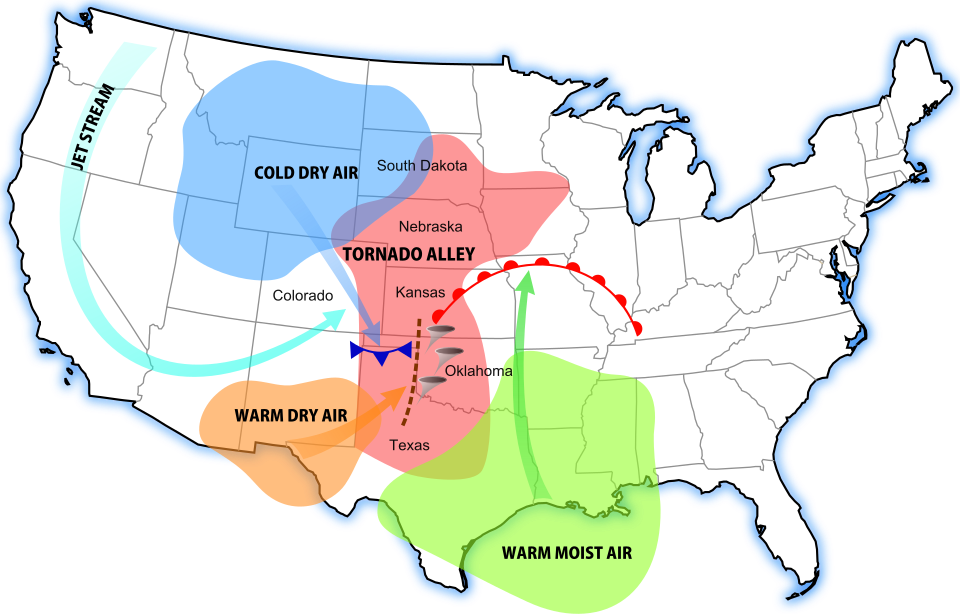
\includegraphics[keepaspectratio]{assets/Tornado_Alley_Diagram.png}}

}

\caption{\label{fig-tornado-alley}This is map highlights the Central
United States, historically referred to as Tornado Alley ({``Tornado
Alley''} 2026).}

\end{figure}%

\begin{figure}

\centering{

\pandocbounded{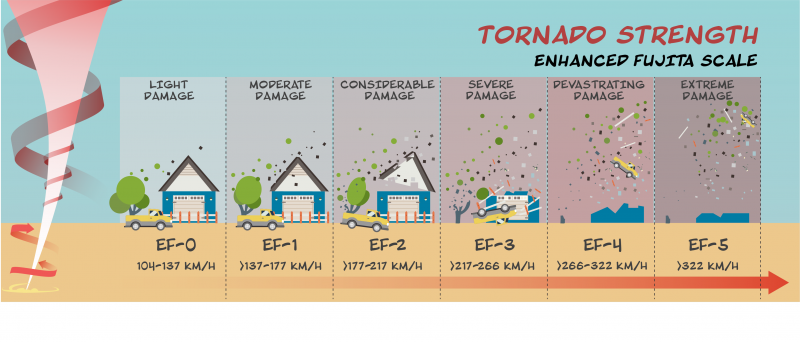
\includegraphics[keepaspectratio]{assets/EF_Scale.png}}

}

\caption{\label{fig-ef-scale}This is a diagram illustrating the
strength, wind speed, and damage typically caused by a tornado at each
classification on the Enhanced Fujita Scale ({``What Is a Tornado? Let's
Talk Science''} 2020).}

\end{figure}%

Additionally, the 75 years of tornado data provided by the NOAA
(DOC/NOAA/NESDIS/NCEI 2026) (which we will later analyze in more detail)
records a small, but not impossible, set of coastal tornado occurrences.
With various species of sharks existing along the Atlantic, Pacific, and
Gulf Coasts of the US, a coastal tornado's ``inventory'' of sharks is
not limited to any specific region (Fisheries 2025). Furthermore, with
an increasing number of tornadoes in atypical regions such as the
Southeastern United States ({``Tornadoes and Climate Change. National
Geographic Education''} 2023), tornadoes' proximity to sharks and
ability to pick them up may be increasing as well.

While there has not been any formal scientific literature that has
studied the likelihood and impacts of tornadoes carrying sharks, one
scholar, Dr.~Kim Martini, entertained the idea and provided an analysis
on the likelihood of a sharknado with her knowledge in marine biology
and physics (Martini 2013). Her analysis resulted in several
conclusions:

\begin{enumerate}
\def\labelenumi{\arabic{enumi}.}
\tightlist
\item
  \textbf{A typical tornado flying over a typical reef could pick up
  about} \textbf{150 sharks}.\\
  \emph{Rationale}: A typical tornado is about 0.1 miles wide, travels
  about 5 miles, and covers an area of 0.5 square miles. A healthy reef
  typically has a shark density of about 300 sharks per square mile.
  However, she notes that one of the largest tornadoes in history was
  2.6 miles wide and traveled 52 miles ({``2004 Hallam Tornado''} 2026),
  making it hypothetically capable of picking up over 40,000 sharks.
\item
  \textbf{It is highly unlikely that a tornado could suck a shark out of
  the water.\\
  }\emph{Rationale}: Tornadic water spouts (see
  Figure~\ref{fig-water-spout}) don't typically suck up water, and
  tagged sharks typically dive deep when there are approaching
  thunderstorms (which can cause tornadoes).
\item
  \textbf{Intense tornadoes are strong enough to keep a shark
  airborne.\\
  }\emph{Rationale}: In the event that a tornado does pick up a shark
  (e.g., a shark hypothetically jumps out of the water as a tornado
  passes over contrary to typical observed behavior), the tornado would
  need to have strong enough vertical wind speeds to combat the force of
  gravity on the shark. With basic physics equations and conservative
  estimates, the minimum upward wind speed required to keep an average
  Great White Shark in the air is 127 mph, which a strong EF4 tornado
  has shown to exhibit. Additionally, smaller sharks are even lighter
  and would require less force to keep them airborne.
\end{enumerate}

\begin{figure}

\centering{

\pandocbounded{
\includegraphics[keepaspectratio]{assets/tornadic-water-spout.}}

}

\caption{\label{fig-water-spout}This is a photo of a tornadic water
spout, essentially a tornado that forms over water or moves from land to
water.}

\end{figure}%

Using this logic, we can assume that EF3 tornadoes (and larger) are
strong enough to pick up small sharks, given that the shark was
transported from the water into the tornado by some odd means. This
transportation of the shark from water to tornado already makes the
occurrence of a sharknado highly unlikely. However, for the purposes of
this report, we will ignore this improbability and assume the physical
transport of sharks is possible, so we can continue analyzing the
geographic and economic frequency of the storm paths themselves.

While tornado intensity is well-studied and the ability for a high
intensity tornado to pick up a shark has been logically proven, there is
a gap in the analysis of the two together. To ensure the profitability
of the insurance agency, we need to know how serious the threat of
sharknadoes is to the insurance agency's bottom line given the warming
climate and shifting trends in tornado activity. Thus, we will use the
historical data found in the NOAA Storm Events Database to evaluate the
likelihood and economic impact of a high-intensity tornado with a
coastal origin moving inland (since these are the types of tornadoes
that have the ability to transport sharks from the ocean) to answer the
research question:

\textbf{\emph{What is the historical frequency, probability, and
economic impact of high-intensity tornadoes (F3, F4, and F5) originating
in coastal areas (Atlantic, Pacific, and Gulf of Mexico) and moving
inland, compared to those following other trajectories?}}

\bookmarksetup{startatroot}

\chapter{Methodology}\label{methodology}

In order to answer the research question (stated at the end of
Chapter~\ref{sec-introduction}), we must

\begin{enumerate}
\def\labelenumi{\arabic{enumi}.}
\tightlist
\item
  Define what qualifies as a storm as a potential ``sharknado''
\item
  Use publicly available historical data to determine the frequency,
  probability, and economic impact of sharknadoes
\end{enumerate}

\section{Defining Sharknado}\label{sec-define-sharknado}

For a tornado to be a potential ``sharknado'', it has to have a few
characteristics:

\begin{enumerate}
\def\labelenumi{\arabic{enumi}.}
\tightlist
\item
  Originates on the coast
\item
  Strong enough to sustain lifting a shark
\item
  Path trajectory moves to the inland
\end{enumerate}

From this, we have to also answer ``What is the `coast' vs what is
`inland'?'' and ``What indicates a tornado is `strong enough' to sustain
lifting a shark?''

\textbf{What is the ``coast'' vs what is ``inland''?}

For the boundary between the coast and open water, the general
definition of a state's coastal zone extends 3 nautical miles into the
ocean from the shore (with some states having their own exceptions). For
the boundary between the coast and the inland, states define their
coastal zone as an extension anywhere from 1,000 feet to 5 miles inland
of the shoreline (Coastal Management n.d.).

Since there is no singular standard, a 3-mile buffer was used to define
the coastal zone along the coastline. This buffer is equally centered
over the coastline, resulting in a zone that extends 1.5 miles into the
ocean and 1.5 miles onto the land. Any point within this buffer zone is
considered the ``Coast'' for the purposes of this analysis. Any point
further inland than the buffer zone is considered ``Inland''.
Section~\ref{sec-coastline-data} details how this coastal buffer zone
was represented in the data.

\textbf{What indicates a tornado is ``strong enough'' to sustain lifting
a shark?}

Based on the physical analysis done by Dr.~Kim Martini (discussed in
Chapter~\ref{sec-introduction}), a strong EF4 tornado has enough
vertical wind speed to keep a great white shark suspended in the air.
Because great white sharks are significantly larger than many other
shark species, it's logical to believe an EF3 tornado has enough
vertical wind speed to suspend much smaller sharks in the air. Since a
shark is a shark, no matter how big or small, this analysis defines
tornadoes classified as (E)F3 and higher on the (Enhanced) Fujita Scale
as ``strong enough'' to sustain lifting a shark.
Section~\ref{sec-aggregate-segments} details how shark-lifting potential
is identified in the data.

\begin{tcolorbox}[enhanced jigsaw, bottomrule=.15mm, colframe=quarto-callout-important-color-frame, colback=white, opacityback=0, toptitle=1mm, leftrule=.75mm, arc=.35mm, title=\textcolor{quarto-callout-important-color}{\faExclamation}\hspace{0.5em}{Important}, bottomtitle=1mm, colbacktitle=quarto-callout-important-color!10!white, coltitle=black, breakable, titlerule=0mm, opacitybacktitle=0.6, rightrule=.15mm, toprule=.15mm, left=2mm]

For the purposes of this analysis, tornado classifications from the
Fujita and Enhanced Fujita Scales were treated synonymously (i.e., EF5 =
F5). Section~\ref{sec-limitations} discusses potential limitations of
this.

\end{tcolorbox}

\section{Data Sources}\label{data-sources}

The primary data for this business report comes from the National
Oceanic and Atmospheric (NOAA) Storm Events Database, which includes 75
years (1950 to 2025) of records of various types of weather events. This
dataset was selected as the primary source because it is one of the most
comprehensive official records of tornadic activity in the United
States, as it provides standardized metrics for storm intensity,
location, and property damage.

Additionally, a shapefile of the 2025 United States coastline was
downloaded into R using the R package \texttt{tigris}. In the analysis,
this shapefile is used to establish the study's geographic boundaries
between coast and the inland.

For more documentation on these data sources, please refer to
Appendix~\ref{sec-data-doc}.

\section{Data Pipeline}\label{data-pipeline}

\begin{tcolorbox}[enhanced jigsaw, bottomrule=.15mm, colframe=quarto-callout-note-color-frame, colback=white, opacityback=0, toptitle=1mm, leftrule=.75mm, arc=.35mm, title=\textcolor{quarto-callout-note-color}{\faInfo}\hspace{0.5em}{Note}, bottomtitle=1mm, colbacktitle=quarto-callout-note-color!10!white, coltitle=black, breakable, titlerule=0mm, opacitybacktitle=0.6, rightrule=.15mm, toprule=.15mm, left=2mm]

\begin{itemize}
\tightlist
\item
  See Figure~\ref{fig-data-pipeline} for a diagram of the full data
  pipeline.
\item
  See Appendix~\ref{sec-tech-methods} for more technical details on this
  methodology.
\end{itemize}

\end{tcolorbox}

\subsection{US Coastline Data}\label{sec-coastline-data}

To implement the above definition of ``Coast'' and ``Inland'' (see
Section~\ref{sec-define-sharknado}), the R package \texttt{tigris} was
used to provide a shapefile of the US Coastline. Once the original
coastline shapefile was imported, it was filtered to only include the
Atlantic, Pacific, and Gulf of Mexico coasts as requested in the
original scenario prompt. The units of the coastline data were converted
from degrees to meters. A 3-mile wide boundary was equally centered over
the coastline, resulting in a zone that extends 1.5 miles into the ocean
and 1.5 miles onto the land. Any point within this buffer zone was
considered the ``Coast'' for the purposes of this analysis. Any point
further inland than the buffer zone was considered ``Inland''. A visual
representation of this data can be seen in
Figure~\ref{fig-coast-buffer}.

\begin{figure}

\centering{

\pandocbounded{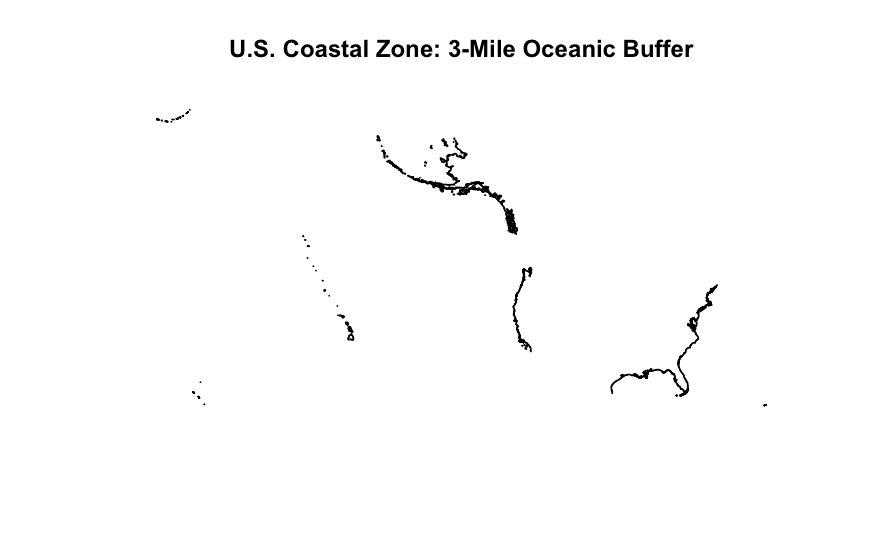
\includegraphics[keepaspectratio]{assets/coast-buffer.png}}

}

\caption{\label{fig-coast-buffer}This is a visual representation of the
US Coastline 3-mile buffer zone generated in the code.}

\end{figure}%

\subsection{NOAA Storm Event Database}\label{noaa-storm-event-database}

\subsubsection{Pre-cleaning \& Filtering}\label{pre-cleaning-filtering}

To begin processing the NOAA Storm Events Database, the data was
filtered to only include tornado weather events. Additionally, any
entries that were missing necessary data were removed.

\subsubsection{Geographical
Classifications}\label{geographical-classifications}

Beginning the work needed to classify tornado path trajectories, each
tornado segment's starting/ending coasts were identified as
``Atlantic'', ``Pacific'', ``Gulf'', or N/A. Each tornado segment's
starting/ending location was also identified as ``Coastal'' or
``Inland''.

\subsubsection{Aggregate Storm Segments}\label{sec-aggregate-segments}

NOAA Storm Events Database is structured so that a single storm may be
recorded as multiple different storm segments. A new storm segment is
created when the tornado enters a new county or zone, resulting in
multiple data rows corresponding to one storm. Thus, segments from the
same storm were identified and stitched back together into a single row
of data.

From here, each tornado's path trajectory was classified as ``Moving
Inland'', ``Moving Coastal'', or ``Other Path'' based on the tornado's
start/end locations. Below further describes the characteristics of each
path trajectory label, along with an illustration in
Figure~\ref{fig-path-trajectories}.

\begin{itemize}
\item
  \textbf{Moving Inland}: tornado originated on the coast and moved
  inland.
\item
  \textbf{Moving Coastal}: tornado originated inland and moved to the
  coast.
\item
  \textbf{Other Path}: tornado originated either inland or on the coast
  and stayed in the same region of origin.
\end{itemize}

\begin{figure}

\centering{

\pandocbounded{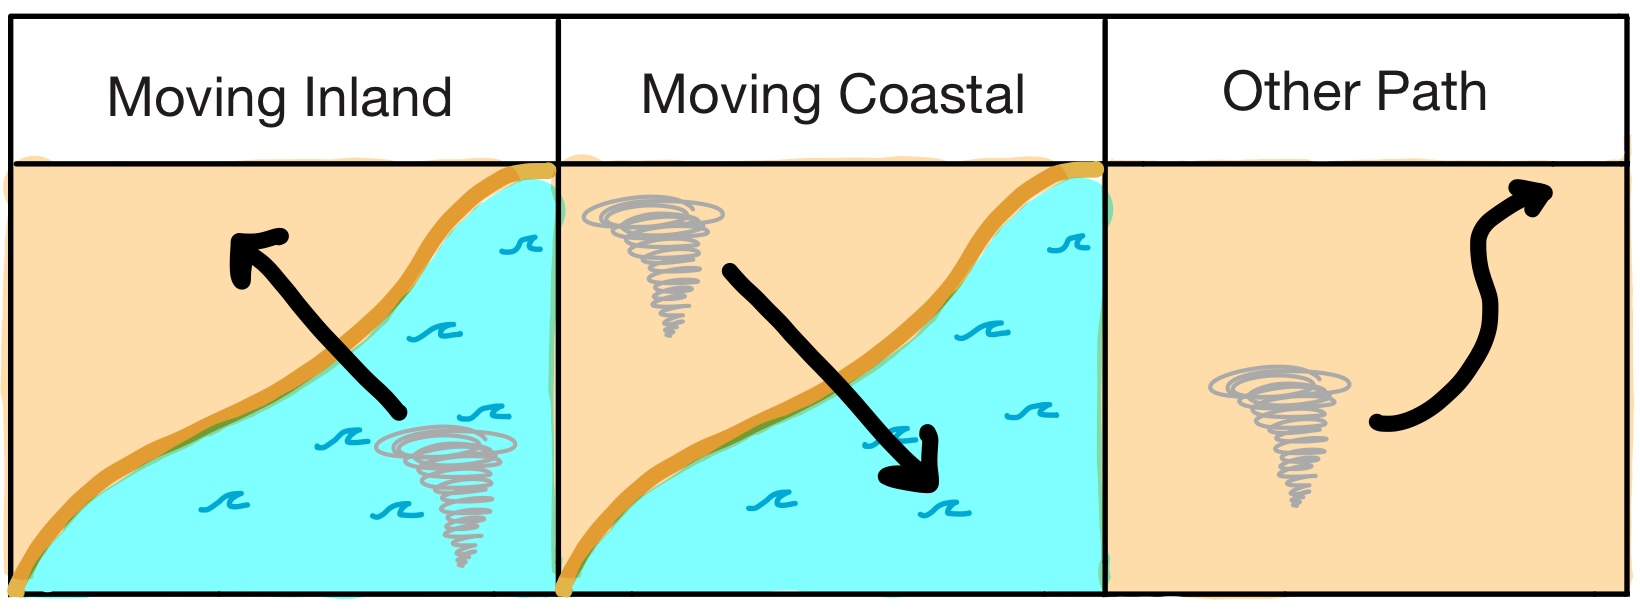
\includegraphics[keepaspectratio]{assets/path-trajectories.jpeg}}

}

\caption{\label{fig-path-trajectories}This is a diagram illustrating the
movement of tornadoes relative to the coast and inland, with path
trajectory labels of ``Moving Inland'', ``Moving Coastal'', and ``Other
Path''.}

\end{figure}%

Finally, each tornado's shark-lifting potential was classified as ``High
Potential'' or ``Low Potential'', based on the storm's (Enhanced) Fujita
Scale RANKING. Below further describes the characteristics of these
labels:

\begin{itemize}
\tightlist
\item
  \textbf{Low Potential}: tornado was given an F1 or F2 rating on the
  (Enhanced) Fujita Scale
\item
  \textbf{High Potential}: tornado was given an F3, F4, or F5 rating on
  the (Enhanced) Fujita Scale
\end{itemize}

\begin{figure}

\centering{

\pandocbounded{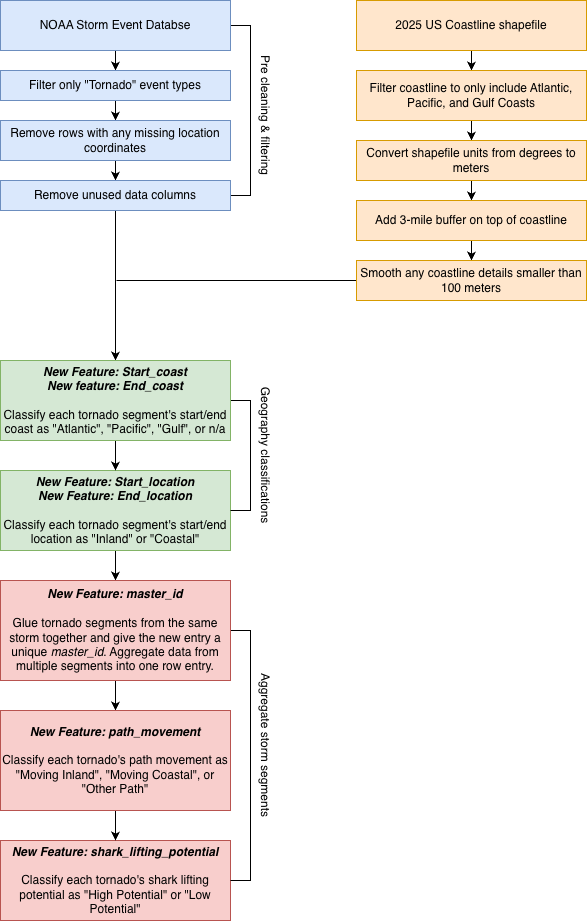
\includegraphics[keepaspectratio]{assets/Sharknado Data Processing.png}}

}

\caption{\label{fig-data-pipeline}This is a diagram illustrating the
steps used to process data and engineer features from the NOAA Storm
Events Database and US Coastline shapefile.}

\end{figure}%

\bookmarksetup{startatroot}

\chapter{Results}\label{results}

\section{Overview of the Study
Population}\label{overview-of-the-study-population}

The analysis of the tornado data from the NOAA Storm Events Database
spans from 1950 through 2025. After combining individual storm segments
into complete tornado events, a total of 31,345 unique tornado events
were identified across the United States. Of these events, 761 started
within the defined 3-mile coastal zone, and only 73 of those ultimately
moved from the coast to the inland. These events were categorized by
their trajectory to determine the potential for transporting sharks. The
population breakdown is as follows in
Table~\ref{tbl-population-breakdown}:

\begin{table}

\caption{\label{tbl-population-breakdown}}

\centering{

\caption*{
{\fontsize{15}{19}\selectfont  Tornado Path Trajectory and Shark-Lifting Potential\fontsize{12}{15}\selectfont } \\ 
{\fontsize{14}{17}\selectfont  1950-2025\fontsize{12}{15}\selectfont }
} 
\fontsize{12.0pt}{14.0pt}\selectfont
\begin{tabular*}{0.8\linewidth}{@{\extracolsep{\fill}}ccc}
\toprule
Shark-Lifting Potential & Event Count & Proportion of Trajectory \\ 
\midrule\addlinespace[2.5pt]
\multicolumn{3}{>{\raggedright\arraybackslash}m{0.8\linewidth}}{\parbox{\linewidth}{{\bfseries Moving Coastal}}} \\[2.5pt] 
\midrule\addlinespace[2.5pt]
High Potential & 2 & 3.2\% \\ 
Low Potential & 60 & 96.8\% \\ 
\midrule\addlinespace[2.5pt]
\multicolumn{3}{>{\raggedright\arraybackslash}m{0.8\linewidth}}{\parbox{\linewidth}{{\bfseries Moving Inland}}} \\[2.5pt] 
\midrule\addlinespace[2.5pt]
High Potential & 2 & 2.7\% \\ 
Low Potential & 71 & 97.3\% \\ 
\midrule\addlinespace[2.5pt]
\multicolumn{3}{>{\raggedright\arraybackslash}m{0.8\linewidth}}{\parbox{\linewidth}{{\bfseries Other Path}}} \\[2.5pt] 
\midrule\addlinespace[2.5pt]
High Potential & 3,799 & 12.2\% \\ 
Low Potential & 27,411 & 87.8\% \\ 
\bottomrule
\end{tabular*}

}

\end{table}%

Initial findings indicate that ``High Potential'' and ``Moving Inland''
events are a minority of total tornado occurrences, with only \textbf{2
total} tornadoes meeting the criteria for ``High Potential'' and
``Moving Inland''. While these unique events are quite rare, they are
certainly not impossible and present a specific kind of threat that
current risk models might be missing.

\section{Path Movement \& Intensity
Analysis}\label{path-movement-intensity-analysis}

To further evaluate the relationship between tornado path trajectory and
intensity, we can visualize the metrics from the previous
Table~\ref{tbl-population-breakdown}. In
Figure~\ref{fig-trajectory-intensity} below, we can see a noticeable
difference in tornadoes that remained completely inland (``Other Path'')
compared to tornadoes that either originated or ended on the coasts.
While ``Moving Inland'' trajectories are the primary focus when
considering the risk of sharknadoes, only \textbf{2.7\%} of these
tornadoes moving from the coast to the inland reached high-potential
intensity. In contrast, ``Other Path'' tornadoes exhibited a much larger
high-potential rate of \textbf{12.2\%}.

\begin{figure}

\centering{

\pandocbounded{\includegraphics[keepaspectratio]{results_files/figure-pdf/fig-trajectory-intensity-1.pdf}}

}

\caption{\label{fig-trajectory-intensity}Categorized all tornadoes by
path trajectory and visualized the percentages of high vs.~low
shark-lifting potential within each path trajectory group.}

\end{figure}%

This suggests that while the ``Moving Inland'' path is geographically
unique, the prime atmospheric conditions needed for F3/F4/F5 tornadoes
are far more prevalent once the storm has moved more inland over land.
For insurance risk modeling, this indicates that while coastal-origin
tornadoes are \emph{capable} of transporting sharks, they are
statistically much less likely to reach the extreme wind speeds of their
inland counterparts.

\section{Regional Risk Distribution}\label{regional-risk-distribution}

To identify likely areas where we could find sharknadoes forming, the
data was segmented by coastal region (Atlantic, Gulf, and Pacific). The
analysis in Figure~\ref{fig-moving-inland-regions} reveals a geographic
imbalance in risk.

The \textbf{Gulf Coast} and \textbf{Atlantic Coast} account for the vast
majority of ``Moving Inland'' events, with each coast responsible for 36
``Moving Inland'' tornadoes. In contrast, the \textbf{Pacific Coast}
only recorded \textbf{1 total} ``Moving Inland'' tornado, which was
identified as ``Low Potential'' intensity. The \textbf{Atlantic Coast}
was the only coastal region that had recorded a ``Moving Inland''
tornado with \textbf{high shark-lifting potential} (2 total occurrences
recorded). Overall, though, the majority of the ``Moving Inland''
tornadoes produced by any of the 3 coasts were identified as ``Low
Potential'' intensity.

\begin{figure}

\centering{

\pandocbounded{\includegraphics[keepaspectratio]{results_files/figure-pdf/fig-moving-inland-regions-1.pdf}}

}

\caption{\label{fig-moving-inland-regions}Categorized only `Moving
Inland' trajectory tornadoes by coastal region and visualized the
percentages of high vs.~low shark-lifting potential within each coastal
region group.}

\end{figure}%

This confirms that sharknado potential is a regional phenomenon, rather
than a national one, with the Atlantic and Gulf Coasts requiring
significantly different actuarial considerations than the West Coast.

\section{Economic Impact}\label{economic-impact}

The final phase of this analysis evaluated the economic impact of
tornadoes based on their path trajectory. Across the 75-year study
period, the total property damage recorded for all events summed to
\textbf{\$3.33B} with an average of \$106,389 per tornado. The summary
of economic impact by tornado trajectory and shark-lifting potential is
in Table~\ref{tbl-trajectory-damage} below:

\begin{table}

\caption{\label{tbl-trajectory-damage}}

\centering{

\caption*{
{\fontsize{15}{19}\selectfont  Economic Impact Analysis by Tornado Trajectory\fontsize{12}{15}\selectfont } \\ 
{\fontsize{14}{17}\selectfont  Property damage and frequency (1950-2025)\fontsize{12}{15}\selectfont }
} 
\fontsize{12.0pt}{14.0pt}\selectfont
\begin{tabular*}{0.9\linewidth}{@{\extracolsep{\fill}}cccc}
\toprule
Shark-Lifting Potential & Total Events & Cumulative Damage & Avg. Damage per Event \\ 
\midrule\addlinespace[2.5pt]
\multicolumn{4}{>{\raggedright\arraybackslash}m{0.9\linewidth}}{\parbox{\linewidth}{{\bfseries Moving Coastal}}} \\[2.5pt] 
\midrule\addlinespace[2.5pt]
Low Potential & 60 & \$41.79M & \$696.53K \\ 
High Potential & 2 & \$9.47M & \$4.73M \\ 
\midrule\addlinespace[2.5pt]
\multicolumn{4}{>{\raggedright\arraybackslash}m{0.9\linewidth}}{\parbox{\linewidth}{{\bfseries Moving Inland}}} \\[2.5pt] 
\midrule\addlinespace[2.5pt]
Low Potential & 71 & \$24.79M & \$349.21K \\ 
High Potential & 2 & \$183.00K & \$91.50K \\ 
\midrule\addlinespace[2.5pt]
\multicolumn{4}{>{\raggedright\arraybackslash}m{0.9\linewidth}}{\parbox{\linewidth}{{\bfseries Other Path}}} \\[2.5pt] 
\midrule\addlinespace[2.5pt]
Low Potential & 27,411 & \$2.58B & \$93.97K \\ 
High Potential & 3,799 & \$682.77M & \$179.72K \\ 
\bottomrule
\end{tabular*}

}

\end{table}%

As visualized in Figure~\ref{fig-trajectory-damage-total} below,
tornadoes following ``Other Path'' trajectories have contributed to
\textbf{97.86\%} of property damage in the last 75 years, which makes
sense since they are the most commonly occurring tornadoes. In contrast,
tornadoes that originated on the coast and moved inland (``Moving
Inland'') have contributed to only \textbf{0.75\%} of all recorded
tornado property damage, with only \textbf{\$183K} in damages resulting
from high shark-lifting potential tornadoes.

\begin{figure}

\centering{

\pandocbounded{\includegraphics[keepaspectratio]{results_files/figure-pdf/fig-trajectory-damage-total-1.pdf}}

}

\caption{\label{fig-trajectory-damage-total}Categorized all tornadoes by
trajectory and visualized the total property damage inflicted by high
vs.~low shark-lifting potential tornadoes within each path trajectory
group.}

\end{figure}%

Based on the visual analysis provided in
Figure~\ref{fig-trajectory-damage-avg}, a hasty conclusion would be that
tornadoes originating inland and moving to the coast (``Moving
Coastal'') result in the most property damage on average. Based on the
calculations, this is technically true. However, it's important to note
that for ``Moving Coastal'' and ``Moving Inland'' tornadoes classified
as high shark-lifting potential, the population consists only of
\textbf{2 total recorded events} for both groups.

\begin{figure}

\centering{

\pandocbounded{\includegraphics[keepaspectratio]{results_files/figure-pdf/fig-trajectory-damage-avg-1.pdf}}

}

\caption{\label{fig-trajectory-damage-avg}Categorized all tornadoes by
trajectory and visualized the average property damage inflicted by high
vs.~low shark-lifting potential tornadoes within each path trajectory
group.}

\end{figure}%

Ultimately, when looking at the tornadoes with sharknado characteristics
(``Moving Inland'' with high shark-lifting potential), only
\textbf{\$183K} in damages has been inflicted in the last 75 years with
an average damage of \textbf{\$91.5K per storm}. From a risk management
perspective, this indicates that while high-intensity coastal-to-inland
events are physically possible, their historical financial impact is
negligible compared to standard inland tornadic activity. For an
insurance agency, these figures suggest that ``Sharknado-style'' events
represent an extremely rare risk rather than a primary cause of annual
losses from catastrophes.

\section{Additional Analysis}\label{additional-analysis}

To further analyze the historical trends of tornado weather intensity,
the (Enhanced) Fujita scale classifications for every recorded tornado
from 1950-2025 were plotted on the line graph shown in
Figure~\ref{fig-historical-intensity-trends} below. In the figure, there
is a clear spike in F0 and F1 tornadoes after 1995. Higher intensity
tornadoes remained relatively constant throughout the time period.

\begin{figure}

\centering{

\pandocbounded{\includegraphics[keepaspectratio]{results_files/figure-pdf/fig-historical-intensity-trends-1.pdf}}

}

\caption{\label{fig-historical-intensity-trends}All tornadoes
categorized by (Enhanced) Fujita category and counts are plotted from
1950-2025}

\end{figure}%

\bookmarksetup{startatroot}

\chapter{Conclusion \& Discussion}\label{conclusion-discussion}

Using 75 years of tornado storm data from the NOAA, we analyzed the
potential for sharknadoes to form in the US and the resulting economic
impacts. We defined a storm as having the potential to produce a
sharknado if it formed on the coast and moved inland (``Moving Inland'')
and had enough strength to carry a shark (category F3, F4, or F5). With
this in mind, we sought to answer the research question:

\textbf{\emph{What is the historical frequency, probability, and
economic impact of high-intensity tornadoes (F3, F4, and F5) originating
in coastal areas (Atlantic, Pacific, and Gulf of Mexico) and moving
inland, compared to those following other trajectories?}}

\section{Frequency \& Probability of
Sharknadoes}\label{frequency-probability-of-sharknadoes}

In the last 75 years, we found that only 2 out of 31,345 recorded
tornadoes exhibited characteristics of ``Moving Inland'' and ``High
Potential'' for shark lifting. Thus, the empirical probability of a
sharknado-like storm is 0.0064\% or approximately 1 in 15,673 U.S.
tornado events, indicating that storms like this are highly rare events.
This frequency is significantly lower than that of high-intensity storms
with a path classification of ``Other Path'', which occur at a rate of
roughly 12.1\%. Given that the concept of a sharknado originated from a
fictional movie, this result was to be expected.

To further reduce concern regarding high shark-lifting potential
tornadoes, we identified only 2 tornadoes with this intensity for both
trajectory categories of ``Moving Inland'' (originating on the coast and
moving inland) and ``Moving Coastal'' (originating inland and moving to
the coast). This was expectedly insignificant compared to the 3,799 high
shark-lifting potential tornadoes in the ``Other Path'' trajectory
category, which makes sense since the inland Tornado Alley region breeds
optimal conditions for high-intensity tornadoes compared to the coasts.

Additionally, the trends visualized in
Figure~\ref{fig-historical-intensity-trends} showed a dramatic spike in
F0 and F1 tornadoes after 1995, and this is almost certainly due to the
modernization of the National Weather Service, specifically the
nationwide deployment of NEXRAD (Next-Generation Radar) Doppler
technology from 1992 to 1997 (Administration 2025). Prior to this
technology, fewer low-intensity tornadoes were recorded because they
occurred in less populated areas or didn't cause enough visible damage
to be reported. It should also be noted that the frequency of
high-intensity storms has remained relatively flat throughout all years
of recorded data. Thus, there is no clear upward trend in storms capable
of producing sharknadoes, even with increasing climate risk.

\section{Regions of Concern}\label{regions-of-concern}

However, as previously mentioned, there has been an upward trend of
tornadoes in atypical regions such as the Southeastern United States
({``Tornadoes and Climate Change. National Geographic Education''}
2023), and perhaps unexpectedly, the majority of tornadoes categorized
as ``Moving Inland'' originated in the Atlantic or Gulf coasts near the
southeastern side of the United States. With the southeast region
already exhibiting these storm characteristics and with climate change
creating volatility in extreme weather events, an increase in storms
with sharknado potential in the southeast is not completely out of the
question.

\section{Economic Impact}\label{economic-impact-1}

In terms of the economic impact of sharknadoes, tornadoes with a path
``Moving Inland'' accounted for only 0.75\% of all recorded tornado
property damage, and even less of that was contributed by high
shark-lifting potential tornadoes moving inland. Over 75 years,
tornadoes ``Moving Inland'' with a high shark-lifting potential resulted
in a total cumulative damage of \$183K and an average of \$91K per
storm, \$14.9K less than the average damage caused by all recorded
tornadoes. Additionally, this was significantly less damage than
tornadoes classified as ``Other Path'' with a high shark-lifting
potential, which resulted in a total cumulative damage of \$682M and an
average of \$179K per storm. This suggests that tornadoes originating in
more typical regions (such as Tornado Alley) have historically caused
far more damage overall and also on a per-storm basis. Thus, an
insurance company covering property damages should be less concerned
with sharknadoes, and more concerned with typical inland tornadoes.

\section{Limitations \& Future Exploration}\label{sec-limitations}

\subsection{Physics Preventing
Sharkadoes}\label{physics-preventing-sharkadoes}

As mentioned in Chapter~\ref{sec-introduction}, it is nearly impossible
for a tornadic water spout to pickup a shark out of the water. This is
because tornadic water spouts don't typically suck up water, and the
behavior of tagged sharks has shown that they usually dive deep when
storms are approaching. So, while this report analyzes the frequency,
probability, and economic impact of sharknado-like storms, the actual
probability of a shark being lifted by a tornado remains close to zero
regardless of storm intensity. This study intentionally overlooks these
mechanical improbabilities to provide a worst-case scenario baseline for
the insurance agency.

\subsection{Dataset Structure}\label{dataset-structure}

The Storm Events Database (DOC/NOAA/NESDIS/NCEI 2026) was the core data
used in this report. One of the major drawbacks of the data's structure
is that a single storm may be recorded as multiple different storm
segments. A new storm segment is created when the tornado enters a new
county or zone, resulting in multiple data rows corresponding to one
storm. Post-1996, segments belonging to the same storm have been
connected using a unique identifier found in the column named
\texttt{EPISODE\_ID}, making the process of connecting segments
relatively straightforward.

However, storms occurring before 1996 do not have a value in the
\texttt{EPISODE\_ID} column. To connect storm segments in this case, we
matched two segments' dates, time, and start/end location coordinates.
Because this is less precise than simply using a unique identifier to
connect storm segments, there could be some room for error in the way
full storm data was aggregated for storms occurring before 1996.

Further analysis could be conducted to compare the pre and post 1996
storms to ensure the difference in segment connection methods doesn't
have any unforeseen effects.

\subsection{Data Validity}\label{data-validity}

The NOAA states that some of the data appearing in the Storm Events
Database may be gathered from sources outside the National Weather
Service. ``An effort is made to use the best available information, but
because of time and resource constraints, information from these sources
may be unverified by the NWS.'' Therefore, the NOAA cautions users that
the NWS does not guarantee accuracy or validity of the information
(National Weather Service n.d.).

\subsection{Data Biases}\label{data-biases}

Due to significant advancements in meteorological technology and
communication systems over the last 75 years, tornado data and records
have certainly improved. In the early decades of the NOAA Storm
Database, tornado records relied heavily on visual confirmation and
manual reporting, which often resulted in under-reporting or less
precise measurements in less populated regions. This could have an
impact on time-series trends because the apparent increase in tornado
frequency over time may be related to improved detection capabilities,
as opposed to increased climate risk.

\subsection{Sample Size \& Temporal
Constraints}\label{sample-size-temporal-constraints}

While the dataset of \(N=31345\) events provides a solid foundation for
analyzing modern tornado trends, the 75-year study period represents a
relatively narrow window in terms of climate history. This limited
temporal scope may not fully capture long-term climate patterns.
Furthermore, the extreme rarity of ``Moving Inland'' and ``High
Potential'' for shark-lifting (\(n=2\)) limits our ability to make
causal inferences or generalizations about the economic impact to future
populations.

\subsection{Storm Intensity Ratings}\label{storm-intensity-ratings}

In the analysis, storm intensity ratings using the Fujita (F) scale and
the Enhanced Fujita (EF) scale were consolidated into a single intensity
metric (i.e., an F5 tornado was treated the same as an EF5 tornado).
While the Enhanced Fujita Scale was derived from the original Fujita
scale, there could be some unforeseen consequences as the scales are
technically different. Treating an F5 tornado as exactly equivalent to
an EF5 tornado may introduce a degree of measurement error, especially
when comparing 20th-century storms to those occurring after the 2007
implementation of the EF system (National Weather Service 2015). This
inconsistency could potentially skew time-series trends, as the criteria
for a ``High Potential'' storm may have shifted slightly between the two
time periods. However, for the purposes of this report, treating the
scales synonymously is the most practical method for initial analysis.

\subsection{Definition of ``Coast'' and ``Other
Path''}\label{definition-of-coast-and-other-path}

In the methodology, a rather arbitrary buffer of 3 miles was used to
geographically and geometrically define the coast. The
\texttt{st\_buffer()} function from the \texttt{sf} package equally
centers the buffer over a line (like the coastline), resulting in a zone
that extends 1.5 miles into the ocean and 1.5 miles onto the land. Since
only 73 out of 31,345 storms were identified as ``Moving Inland''
(originating on the coast and traveling inland), further analysis could
be conducted by testing different buffer values, especially larger ones,
to see if the recorded number of ``Moving Inland'' storms is affected.

Additionally, storm trajectories classified as ``Other Path'' included
storms that started and remained inland, along with storms that started
on the coast and remained on the coast. However, with the 3-mile buffer
zone, storms that started on the coast and remained on the coast could
technically include storms that originated within the 1.5-mile extension
into the ocean and ended on land within the 1.5-mile extension inland.
Thus, decreasing the buffer zone's size or moving the buffer zone closer
to the water could shift some ``Other Path'' classifications to ``Moving
Inland''. If this change were made, it is possible the results would
show an increase in sharknado frequency.

\section{Going Forward}\label{going-forward}

Ultimately, with such a small number of recorded storms exhibiting
characteristics expected of a sharknado along with relatively small
amounts of inflicted damage, the insurance agency should not be
concerned with sharknadoes having an impact on their bottom line. Though
with climate change having an impact on extreme weather events, it
wouldn't hurt the agency to periodically track if there is a continuing
trend in storms forming in the southeastern region of the US, which is
closer to the Gulf and Atlantic Coasts.

\begin{tcolorbox}[enhanced jigsaw, bottomrule=.15mm, colframe=quarto-callout-tip-color-frame, colback=white, opacityback=0, toptitle=1mm, leftrule=.75mm, arc=.35mm, title=\textcolor{quarto-callout-tip-color}{\faLightbulb}\hspace{0.5em}{Action Items}, bottomtitle=1mm, colbacktitle=quarto-callout-tip-color!10!white, coltitle=black, breakable, titlerule=0mm, opacitybacktitle=0.6, rightrule=.15mm, toprule=.15mm, left=2mm]

\begin{itemize}
\tightlist
\item
  \textbf{Treat Marine-Origin Events as Rare Events:} High-intensity
  ``Moving Inland'' tornadoes remain an extreme statistical rarity, with
  only two recorded occurrences in 75 years. These should be categorized
  as low-probability, ``long-tail'' risks rather than primary drivers of
  annual catastrophe loss.
\item
  \textbf{Maintain Standard Inland Risk Models}: With 97.86\% of
  historical property damage occurring in ``Other Path'' trajectories,
  the agency should continue prioritizing traditional inland tornado
  risk models over specialized ``Sharknado'' or marine-origin coverages.
\item
  \textbf{Monitor Southeast Regional Shifts:} While national
  ``Sharknado'' risk is negligible, the Gulf and Atlantic coasts account
  for the vast majority of coastal-to-inland storm paths. The agency
  should periodically track storm trends in the Southeastern U.S., where
  climate change \emph{may} be increasing the frequency of atypical,
  high-intensity coastal events.
\end{itemize}

\end{tcolorbox}

\bookmarksetup{startatroot}

\chapter*{References}\label{references}
\addcontentsline{toc}{chapter}{References}

\markboth{References}{References}

\phantomsection\label{refs}
\begin{CSLReferences}{1}{0}
\bibitem[\citeproctext]{ref-2004HallamTornado2026}
{``2004 Hallam Tornado.''} 2026. In \emph{Wikipedia}.
\url{https://en.wikipedia.org/w/index.php?title=2004_Hallam_tornado&oldid=1345145456}.

\bibitem[\citeproctext]{ref-NextGenerationWeather}
Administration, Federal Aviation. 2025. {``Next Generation Weather Radar
({NEXRAD}). Federal Aviation Administration {\textbar} United States
Department of Transportation.''} September 16, 2025.
\url{https://www.faa.gov/air_traffic/weather/nexrad}.

\bibitem[\citeproctext]{ref-bureauTIGERLineShapefiles}
Bureau, US Census. 2025a. {``{TIGER}/Line Shapefiles and {TIGER}/Line
Files Technical Documentation. Census.gov.''} September 17, 2025.
\url{https://www.census.gov/programs-surveys/geography/technical-documentation/complete-technical-documentation/tiger-geo-line.html}.

\bibitem[\citeproctext]{ref-bureauCensusMappingFiles}
---------. 2025b. {``Census Mapping Files. Census.gov.''} September 26,
2025. \url{https://www.census.gov/geographies/mapping-files.html}.

\bibitem[\citeproctext]{ref-NationalCoastalZone}
Coastal Management, Office for. n.d. {``Coastal Zone Management
Programs. Office for Coastal Management {\textbar} {NOAA}.''} Accessed
April 13, 2026. \url{https://coast.noaa.gov/czm/mystate/}.

\bibitem[\citeproctext]{ref-StormEventsDatabasea}
DOC/NOAA/NESDIS/NCEI. 2026. {``Storm Events Database {\textbar} National
Centers for Environmental Information.''}
https://www.ncei.noaa.gov/pub/data/swdi/stormevents/csvfiles/.
\url{https://www.ncei.noaa.gov/stormevents/ftp.jsp}.

\bibitem[\citeproctext]{ref-Sharknado}
Ferrante, Anthony. 2013. \emph{Sharknado}. Syfy.

\bibitem[\citeproctext]{ref-fisheriesSharksAtlanticGulf2025}
Fisheries, NOAA. 2025. {``Sharks in Atlantic, Gulf, and Caribbean
Coastal Waters. {NOAA} Fisheries.''} {NOAA} Fisheries. February 26,
2025.
\url{https://www.fisheries.noaa.gov/atlantic-highly-migratory-species/sharks-atlantic-gulf-and-caribbean-coastal-waters}.

\bibitem[\citeproctext]{ref-martiniRecipeSharknadoDeep2013}
Martini, Dr. Kim. 2013. {``Recipe for a Sharknado {\textbar} Deep Sea
News. Deep Sea News.''} August 9, 2013.
\url{https://deepseanews.com/2013/08/recipe-for-a-sharknado/}.

\bibitem[\citeproctext]{ref-usdepartmentofcommerceEFScale}
National Weather Service, NOAA's. 2015. {``{EF} Scale. National Weather
Service.''} {NOAA}'s National Weather Service. March 27, 2015.
\url{https://www.weather.gov/lsx/enhancedfujitascale}.

\bibitem[\citeproctext]{ref-centerNOAAsNWSStorm}
---------. 2025. {``The Enhanced Fujita Scale ({EF} Scale). Storm
Prediction Center.''} {NOAA}'s National Weather Service. May 21, 2025.
\url{https://www.spc.noaa.gov/efscale/}.

\bibitem[\citeproctext]{ref-StormEventsDatabaseb}
---------. n.d. {``Storm Events Database - {FAQ}. National Centers for
Environmental Information.''} Accessed April 9, 2026.
\url{https://www.ncei.noaa.gov/stormevents/faq.jsp}.

\bibitem[\citeproctext]{ref-TornadoAlley2026}
{``Tornado Alley.''} 2026. In \emph{Wikipedia}.
\url{https://en.wikipedia.org/w/index.php?title=Tornado_Alley&oldid=1339195322}.

\bibitem[\citeproctext]{ref-TornadoesClimateChange}
{``Tornadoes and Climate Change. National Geographic Education.''} 2023.
October 19, 2023.
\url{https://education.nationalgeographic.org/resource/tornadoes-and-climate-change}.

\bibitem[\citeproctext]{ref-TigrisPackageRDocumentation}
Walker, Kylie. 2025. {``Tigris Package - {RDocumentation}.
Rdocumentation.''} April 16, 2025.
\url{https://www.rdocumentation.org/packages/tigris/versions/2.2.1}.

\bibitem[\citeproctext]{ref-WhatTornadoLets2020}
{``What Is a Tornado? Let's Talk Science.''} 2020. February 26, 2020.
\url{https://letstalkscience.ca/educational-resources/stem-explained/what-a-tornado}.

\end{CSLReferences}

\cleardoublepage
\phantomsection
\addcontentsline{toc}{part}{Appendices}
\appendix

\chapter{Technical Methodology}\label{sec-tech-methods}

\section{Data Pipeline}\label{data-pipeline-1}

\begin{tcolorbox}[enhanced jigsaw, bottomrule=.15mm, colframe=quarto-callout-note-color-frame, colback=white, opacityback=0, toptitle=1mm, leftrule=.75mm, arc=.35mm, title=\textcolor{quarto-callout-note-color}{\faInfo}\hspace{0.5em}{Note}, bottomtitle=1mm, colbacktitle=quarto-callout-note-color!10!white, coltitle=black, breakable, titlerule=0mm, opacitybacktitle=0.6, rightrule=.15mm, toprule=.15mm, left=2mm]

See Figure~\ref{fig-data-pipeline} for a diagram of the full data
pipeline.

\end{tcolorbox}

\subsection{US Coastline Data}\label{sec-coastline-data}

To implement the above definition of ``Coast'' and ``Inland'' (see
Section~\ref{sec-define-sharknado}), the R package \texttt{tigris} was
used to provide a shapefile of the US Coastline. Once the original
coastline shapefile was imported, it was filtered to only include the
Atlantic, Pacific, and Gulf of Mexico coasts as requested in the
original scenario prompt. The units of the coastline data were converted
from degrees to meters using the \texttt{st\_transform} function from
the \texttt{tigris} package prepare for a meter-based buffer. Using the
\texttt{st\_buffer} function from the \texttt{tigris} package, a 3-mile
(4828 meter) buffer was equally centered over the coastline, resulting
in a zone that extends 1.5 miles into the ocean and 1.5 miles onto the
land. Any point within this buffer zone is considered the ``Coast'' for
the purposes of this analysis. Any point further inland than the buffer
zone is considered ``Inland''. Finally, any coastline details smaller
than 100m were smoothed using the \texttt{st\_simplify} function from
the \texttt{tigris} package to increase computational efficiency without
sacrificing regional accuracy. A visual representation of this data can
be seen in Figure~\ref{fig-coast-buffer}.

\begin{figure}

\centering{

\pandocbounded{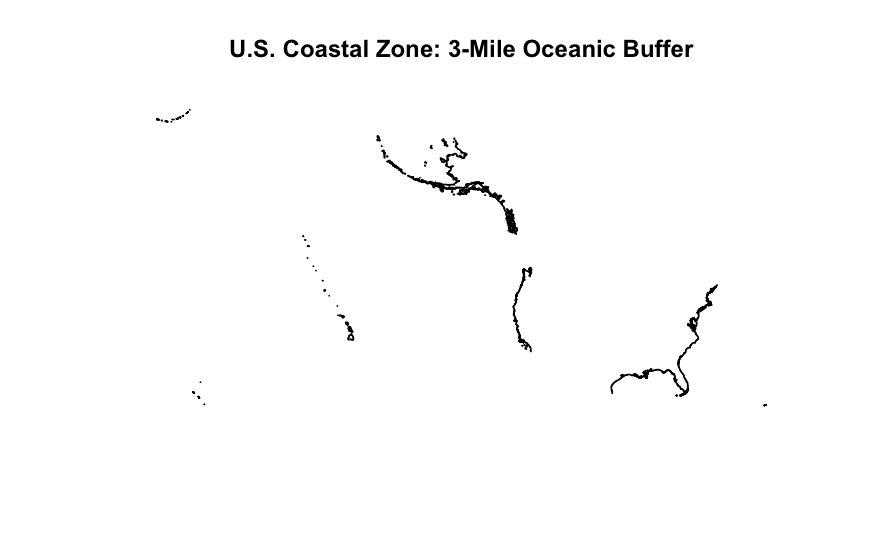
\includegraphics[keepaspectratio]{assets/coast-buffer.png}}

}

\caption{\label{fig-coast-buffer}This is a visual representation of the
US Coastline 3-mile buffer zone generated in the code.}

\end{figure}%

\subsection{NOAA Storm Event
Database}\label{noaa-storm-event-database-1}

\subsubsection{Pre-cleaning \&
Filtering}\label{pre-cleaning-filtering-1}

To begin processing the NOAA Storm Events Database, we \texttt{filter}
the data to only include events that are
\texttt{EVENT\_TYPE\ =\ Tornado}. Additionally, any entries that are
missing location coordinates for the features \texttt{BEGIN\_LAT},
\texttt{BEGIN\_LON}, \texttt{END\_LAT}, \texttt{END\_LON} were removed
since we wouldn't be able to calculate their path trajectories. Finally,
any features \textbf{not} in the following list were removed since they
were not needed for the analysis:

\begin{itemize}
\item
  \texttt{EPISODE\_ID}
\item
  \texttt{EVENT\_ID}
\item
  \texttt{YEAR}
\item
  \texttt{MONTH\_NAME}
\item
  \texttt{BEGIN\_DATE\_TIME}
\item
  \texttt{STATE}
\item
  \texttt{BEGIN\_LAT}
\item
  \texttt{BEGIN\_LON}
\item
  \texttt{END\_LAT}
\item
  \texttt{END\_LON}
\item
  \texttt{TOR\_F\_SCALE}
\item
  \texttt{DAMAGE\_PROPERTY}
\end{itemize}

\subsubsection{Geographical
Classifications}\label{geographical-classifications-1}

Beginning the work needed to classify tornado path trajectories, we
started by engineering two new features \texttt{Start\_coast} and
\texttt{End\_coast}, which classify the tornado segment as
starting/ending in the ``Atlantic'', ``Pacific'', ``Gulf'', or N/A. This
is done by comparing the \texttt{BEGIN\_LAT}, \texttt{BEGIN\_LON},
\texttt{END\_LAT}, \texttt{END\_LON} features to the modified coastline
shapefile.

From here, two more features were created \texttt{Start\_location} and
\texttt{End\_location}, which classify the tornado segment as
starting/ending on the ``Coastal'' or ``Inland'' based on whether the
\texttt{Start\_coast} and \texttt{End\_coast} columns are empty for the
feature.

\subsubsection{Aggregate Storm Segments}\label{sec-aggregate-segments}

NOAA Storm Events Database is structured so that a single storm may be
recorded as multiple different storm segments. A new storm segment is
created when the tornado enters a new county or zone, resulting in
multiple data rows corresponding to one storm. Post-1996, segments
belonging to the same storm have been connected using a unique
identifier found in the column named \texttt{EPISODE\_ID}, making the
process of connecting segments relatively straightforward. However,
storms occurring before 1996 do not have a value in the
\texttt{EPISODE\_ID} column. To connect storm segments from this era, we
matched segments' dates, times, and start/end location coordinates.

Once tornado segments were stitched together into one full tornado
entry, a new feature, \texttt{master\_id}, was created to serve as an
ultimate unique identifier for each full tornado. For pre-1996 storms,
the unique \texttt{master\_id} was formatted as
\texttt{YEAR\ MONTH\_NAME\ STATE\ BEGIN\_LAT\ BEGIN\_LON} (e.g., 1950
September OKLAHOMA 35 -96.25). For post-1996 storms, the
\texttt{EPISODE\_ID} was used for the \texttt{master\_id} since it is
already a unique identifier for each full storm.

Because multiple tornado segments were stitched together, we needed to
consolidate all of the data from each of the segments into a single
entry. The following list summarizes how the data was consolidated for
each feature:

\begin{itemize}
\tightlist
\item
  \texttt{YEAR}: use the year of the first segment
\item
  \texttt{MONTH\_NAME}: use the month name from the first segment
\item
  \texttt{Beginning\_State}: use the state of the first segment
\item
  \texttt{End\_State}: use the state of the last segment
\item
  \texttt{Start\_location}: use the start location of the first segment
\item
  \texttt{End\_location}: use the end location of the last segment
\item
  \texttt{Start\_coast}: use the start coast of the first segment
\item
  \texttt{End\_coast}: use the end coast of the last segment
\item
  \texttt{TOR\_F\_SCALE\_MAX}: maximum (Enhanced) Fujita scale ranking
  across all segments
\item
  \texttt{Total\_Damage}: sum of \texttt{DAMAGE\_PROPERTY} across all
  segments
\end{itemize}

From here, a new feature \texttt{path\_movement} was created, which
classifies the path trajectory of the full tornado as ``Moving Inland'',
``Moving Coastal'', or ``Other Path'' based on the
\texttt{Start\_location} and \texttt{End\_location} features. Below
further describes the characteristics of each path trajectory, along
with an illustration in Figure~\ref{fig-path-trajectories}.

\begin{itemize}
\item
  \textbf{Moving Inland}: tornado originated on the coast and moved
  inland.
\item
  \textbf{Moving Coastal}: tornado originated inland and moved to the
  coast.
\item
  \textbf{Other Path}: tornado originated either inland or on the coast
  and stayed in the same region of origin.
\end{itemize}

\begin{figure}

\centering{

\pandocbounded{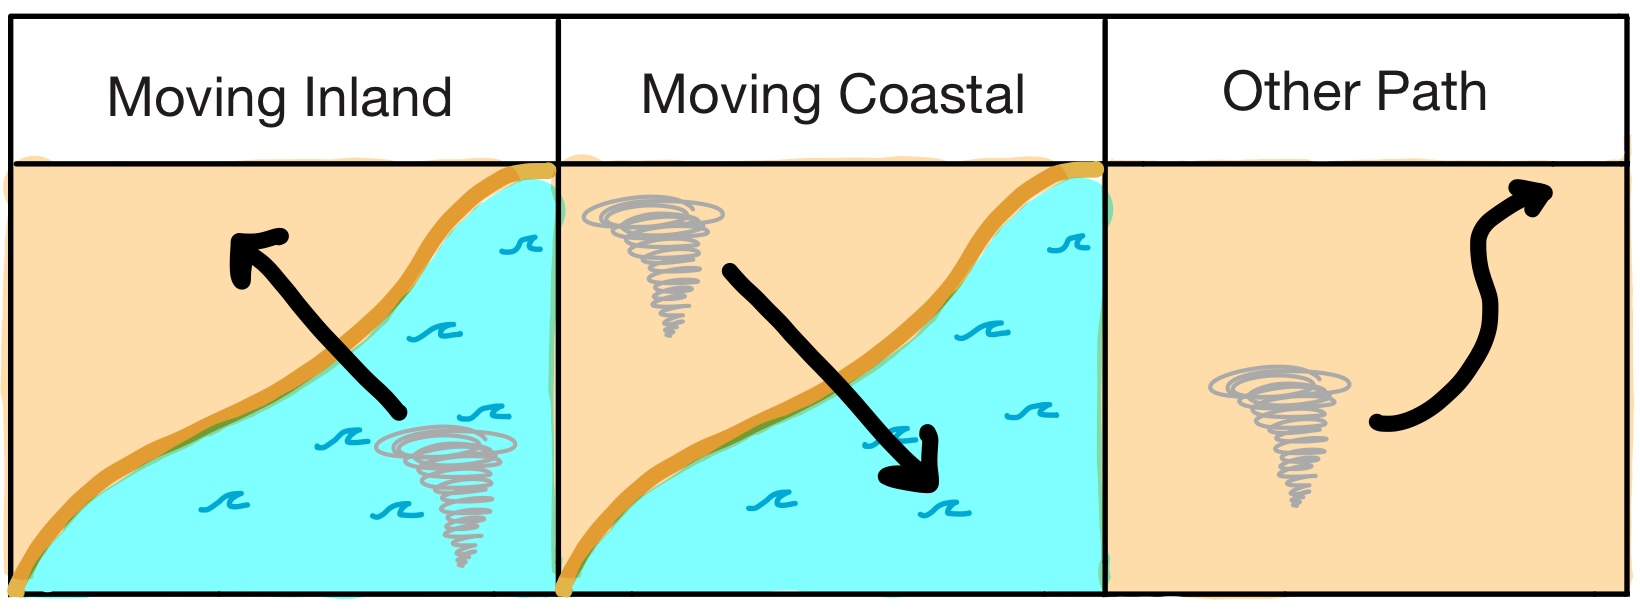
\includegraphics[keepaspectratio]{assets/path-trajectories.jpeg}}

}

\caption{\label{fig-path-trajectories}This is a diagram illustrating the
movement of tornadoes relative to the coast and inland, with path
trajectory labels of ``Moving Inland'', ``Moving Coastal'', and ``Other
Path''.}

\end{figure}%

Finally, a new feature \texttt{shark\_lifting\_potential} was created,
which classifies the shark-lifting potential of the full tornado as
``High Potential'' or ``Low Potential'', based on the
\texttt{TOR\_F\_SCALE\_MAX} feature. Below further describes the
characteristics of these labels:

\begin{itemize}
\tightlist
\item
  \textbf{Low Potential}: tornado was given an F1 or F2 rating on the
  (Enhanced) Fujita Scale
\item
  \textbf{High Potential}: tornado was given an F3, F4, or F5 rating on
  the (Enhanced) Fujita Scale
\end{itemize}

\begin{figure}

\centering{

\pandocbounded{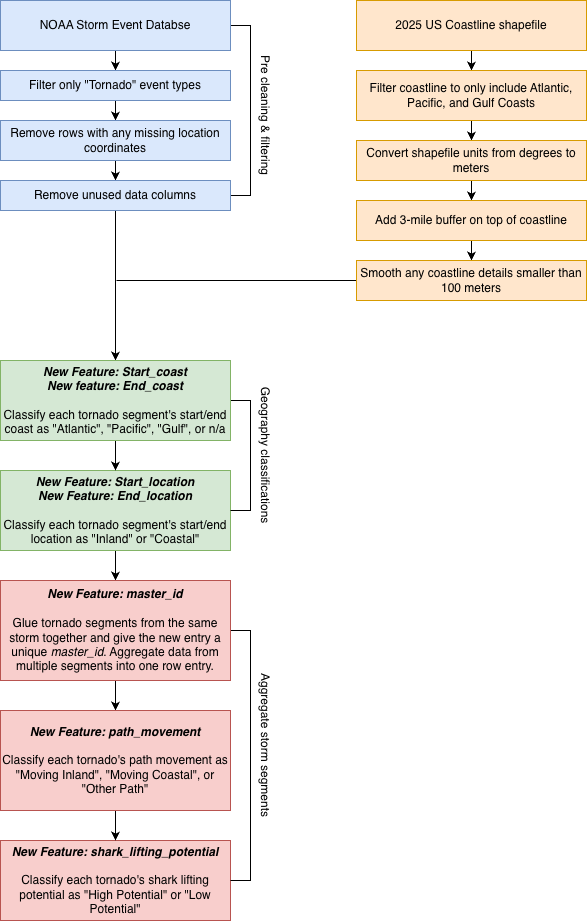
\includegraphics[keepaspectratio]{assets/Sharknado Data Processing.png}}

}

\caption{\label{fig-data-pipeline}This is a diagram illustrating the
steps used to process data and engineer features from the NOAA Storm
Events Database and US Coastline shapefile.}

\end{figure}%

\chapter{Data Documentation}\label{sec-data-doc}

\section{NOAA Storm Events Database}\label{noaa-storm-events-database}

The Storm Events Database (DOC/NOAA/NESDIS/NCEI 2026) was entered by the
National Centers for Environmental Information (NCEI) under the National
Oceanic and Atmospheric Administration (NOAA), which receives data from
the National Weather Service (NWS). This data set records the occurrence
of intense storms and weather phenomena that have caused loss of life,
injuries, significant property damage, and/or disruption to commerce.
Also documented are rare, unusual weather phenomena that generate media
attention, along with other record maximum or minimum meteorological
events that occur in connection with another event. This data was
collected and entered to create the official NOAA Storm Data publication
and document significant weather events.

\subsection{Collection}\label{collection}

All data in the set was collected between January 1950 and October 2025.
The National Weather Service receives its information from a variety of
sources, which include but are not limited to: county, state, and
federal emergency management officials, local law enforcement officials,
skywarn spotters, NWS damage surveys, newspaper clipping services, the
insurance industry, and the general public, among others. Because the
NWS receives information from multiple sources, details are not provided
on measurement instruments. New data for a given month is updated in the
database 75-90 days after the end of that month.

\subsection{Structure \& Formatting}\label{structure-formatting}

Since 2006, NWS has supplied NCEI with data in the form of CSV text
files that are imported into NCEI's Storm Events Database. In the data
set, each year of data has three different CSV files related to each,
where each file contains events from that given year and is
characterized by one of three data categories/file types: Event Details,
Locations, and Fatalities. This analysis only used the ``Event Details''
file for each year of data, as it contained all the needed data columns
for analysis. Notable columns that span across the three file types
include start and end date/times, location (state and periodic
latitude/longitude coordinates), event type (e.g., tornado), intensity,
and fatalities/damage.

Dates are recorded as \emph{YYYYMM} or \emph{DD-MM-YY HH:MM:SS}.
Location coordinates are formatted in decimal degrees. Tornado
intensities are ranked using the Fujita (F) scale or the Enhanced Fujita
(EF) scale, which are categorical variables (F0-F5 or EF0-EF5).

Another notable characteristic of the data's structure is that a single
storm may be recorded as multiple different storm segments. A new storm
segment is created when the tornado enters a new county or zone,
resulting in multiple data rows corresponding to one storm. For pre-1996
storms, there was no connecting identifier across storm segments
belonging to the same full storm. For post-1996 storms, the
\texttt{EPISODE\_ID} was used as the connecting identifier across storm
segments belonging to the same full storm.

As an additional note, the Storm Events Database main page states that,
``NCEI has performed data reformatting and standardization of event
types but has not changed any data values for locations, fatalities,
injuries, damage, narratives, and any other event-specific
information.''

\href{https://www.ncei.noaa.gov/pub/data/swdi/stormevents/csvfiles/}{Repository}\\
\href{https://www.ncei.noaa.gov/pub/data/swdi/stormevents/csvfiles/README}{README}
- information on the naming conventions of the files.\\
\href{https://www.ncei.noaa.gov/pub/data/swdi/stormevents/csvfiles/Storm-Data-Export-Format.pdf}{Storm
Data Export Format} - description of columns across Event Details Files,
Location Files, and Fatality Files

\subsection{Data Validation \& Quality
Control}\label{data-validation-quality-control}

According to the ``Storm Data FAQ Page'' (National Weather Service
n.d.), ``An effort is made to use the best available information, but
because of time and resource constraints, information from these sources
may be unverified by the NWS. Therefore, when using information from
Storm Data, customers should be cautious as the NWS does not guarantee
the accuracy or validity of the information.''

\subsection{Data Reuse}\label{data-reuse}

As a product of the U.S. Federal Government (Department of Commerce),
this data is in the public domain and is free to use for research
without a paid license.

\section{U.S. Census Mapping Files}\label{u.s.-census-mapping-files}

\texttt{tigris} is an R package that allows users to directly download
and use TIGER/Line shapefiles from the US Census Bureau (Walker 2025).
This analysis utilized \texttt{tigris} to retrieve a current shapefile
of the 2025 United States coastline. In the analysis, this shapefile is
used to establish the study's geographic boundaries between the coast
and the inland.

The Census Mapping Files are entered by the U.S. Census Bureau. Broadly,
these files are considered as Geographic Information System (GIS)
mapping files, which contain spatial data encoded into a file format.
Examples of these types of files include Shapefiles, KML, and File
Geodatabase files. For this report, the ``Coastline National shapefile''
held data points that mapped the coastline of the U.S. TIGER stands for
Topologically Integrated Geographic Encoding and Referencing system and
represents the U.S. Census Bureau's geographical spatial data.

The purpose of the U.S. Census TIGER/Line Shapefiles is for
``statistical data collection and tabulation purposes only. Their
depiction and designation for statistical purposes does not constitute a
determination of jurisdictional authority or rights of ownership or
entitlement and are not legal land descriptions,'' {[}Bureau (2025a)\}.
An additional disclaimer: ``TIGER/Line Shapefiles do not include
demographic data, but they do contain geographic entity codes (GEOIDs)
that can be linked to the Census Bureau's demographic data,'' (Bureau
2025b).

More technical documentation regarding the U.S. Census Bureau TIGER/Line
Shapefiles can be found at
\href{https://www.census.gov/programs-surveys/geography/technical-documentation/complete-technical-documentation/tiger-geo-line.html}{TIGER/Line
Shapefiles and TIGER/Line Files Technical Documentation}.

\subsection{Collection}\label{collection-1}

The Census Bureau maintains the MAF/TIGER System (Master Address
File/Topologically Integrated Geographic Encoding and Referencing)
through several sources, such as federal, state, and local governments,
the Boundary and Annexation Survey (BAS), aerial imagery and fieldwork,
and historical sources (Bureau 2025a).

\subsection{Structure \& Formatting}\label{structure-formatting-1}

The Coastlines Shapefile is a national-level dataset provided as a
zipped archive containing seven specific GIS file types, such as .shp
for geometry and .dbf for tabular attributes. The data is formatted
using the GCS NAD83 coordinate system with six decimal places of
precision, ensuring high spatial accuracy for coastal mapping. Within
the attribute table, each linear feature is standardized using the L4150
MAF/TIGER Feature Class Code and includes a primary name field
corresponding to the bordering body of water (Bureau 2025a).

\subsection{Data Validation \& Quality
Control}\label{data-validation-quality-control-1}

The Census Bureau maintains data quality through the Boundary and
Annexation Survey (BAS), an annual program that verifies legal
boundaries with tribal, state, and local governments to ensure the
MAF/TIGER System remains current. Additionally, the Bureau employs
automated validation edits and provides a Spatial Metadata Identifier
(SMID) for every line segment, allowing users to track the specific
source and horizontal accuracy of the data (Bureau 2025a).

\subsection{Data Reuse}\label{data-reuse-1}

``Copyright protection is not available for any work of the United
States Government (Title 17 U.S.C., Section 105). Thus, you are free to
reproduce census materials as you see fit. We would ask, however, that
you cite the Census Bureau as the source,'' (Bureau 2025a).




\end{document}
